\documentclass[a4paper,11pt]{report}	
\usepackage[T1]{fontenc}
\usepackage[utf8]{inputenc}
\usepackage[brazilian]{babel}
\usepackage{enumerate}
\usepackage{graphicx, wrapfig}
\usepackage[leftcaption]{sidecap}
\title{mechendo no latex quatro.0}
\author{Xusp} 

\begin{document}
\maketitle
\tableofcontents
\listoffigures.
\chapter{Imagens}
\section{}
%\begin{figure}[htpb]
Essa imagem ta com [scale=0.2]
\begin{SCfigure}[0.25][h]
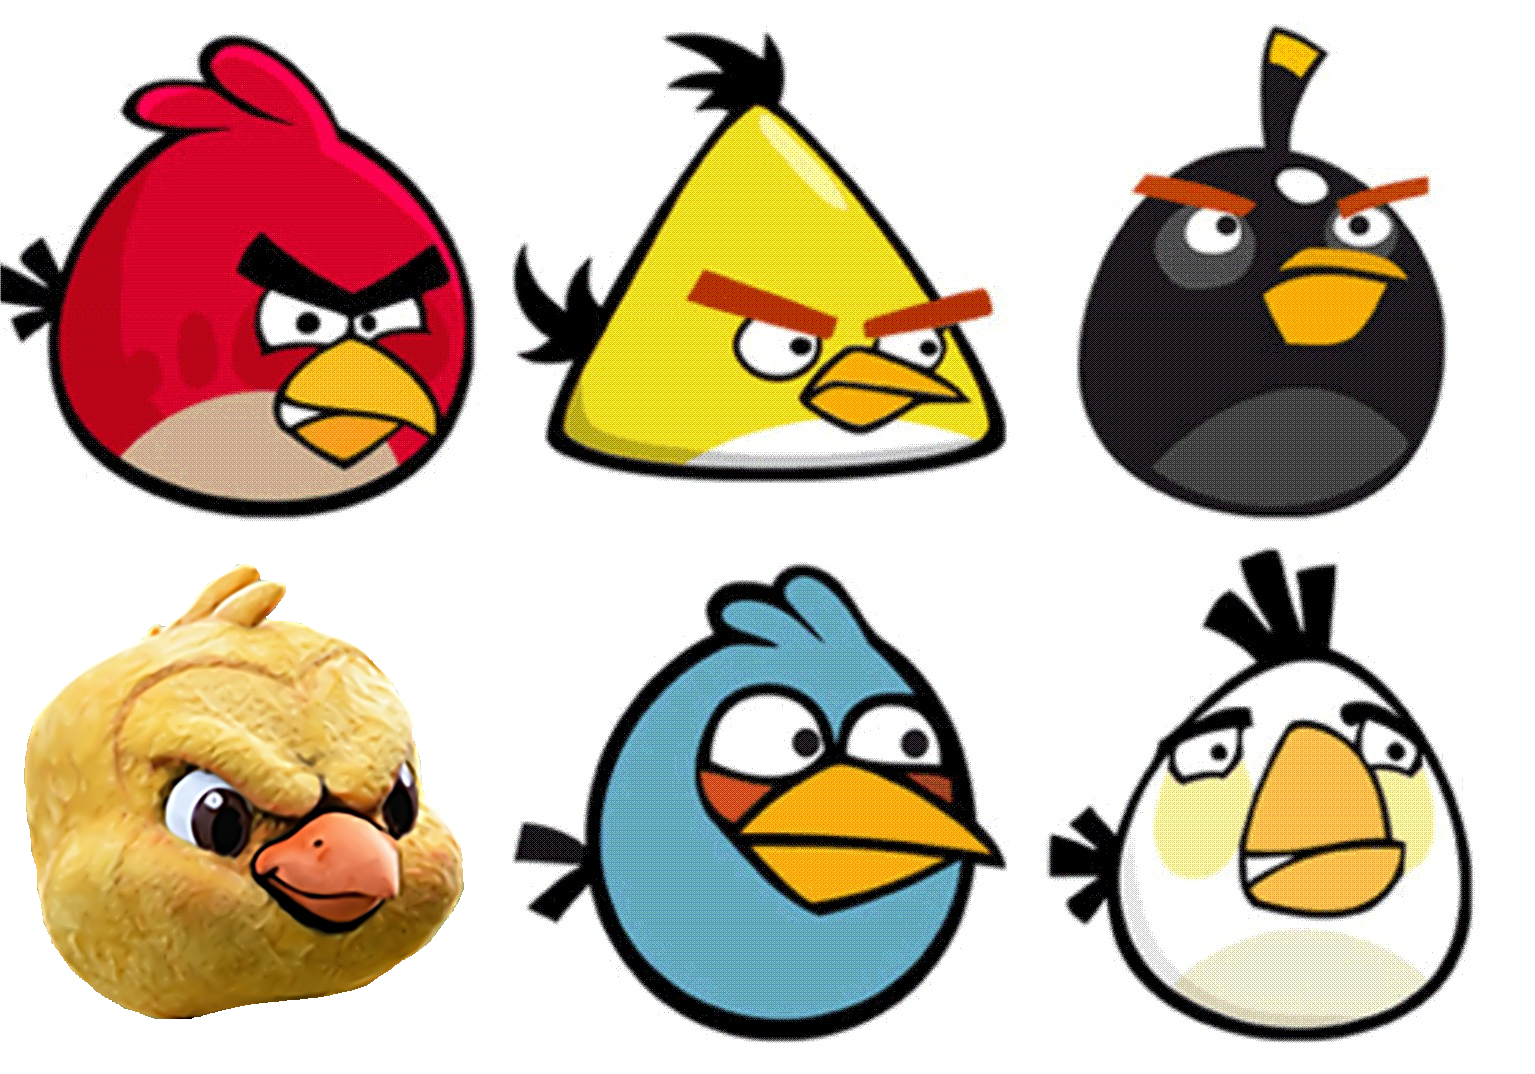
\includegraphics[scale=0.2]{Pistola_Birds.png}
\caption{Pistola Birds um}\label{imagemprimeira}
\end{SCfigure}
%\end{figure}
\section{}
\begin{figure}[htpb]
Essa imagem ta com [height=4cm, width=10]
\begin{center}
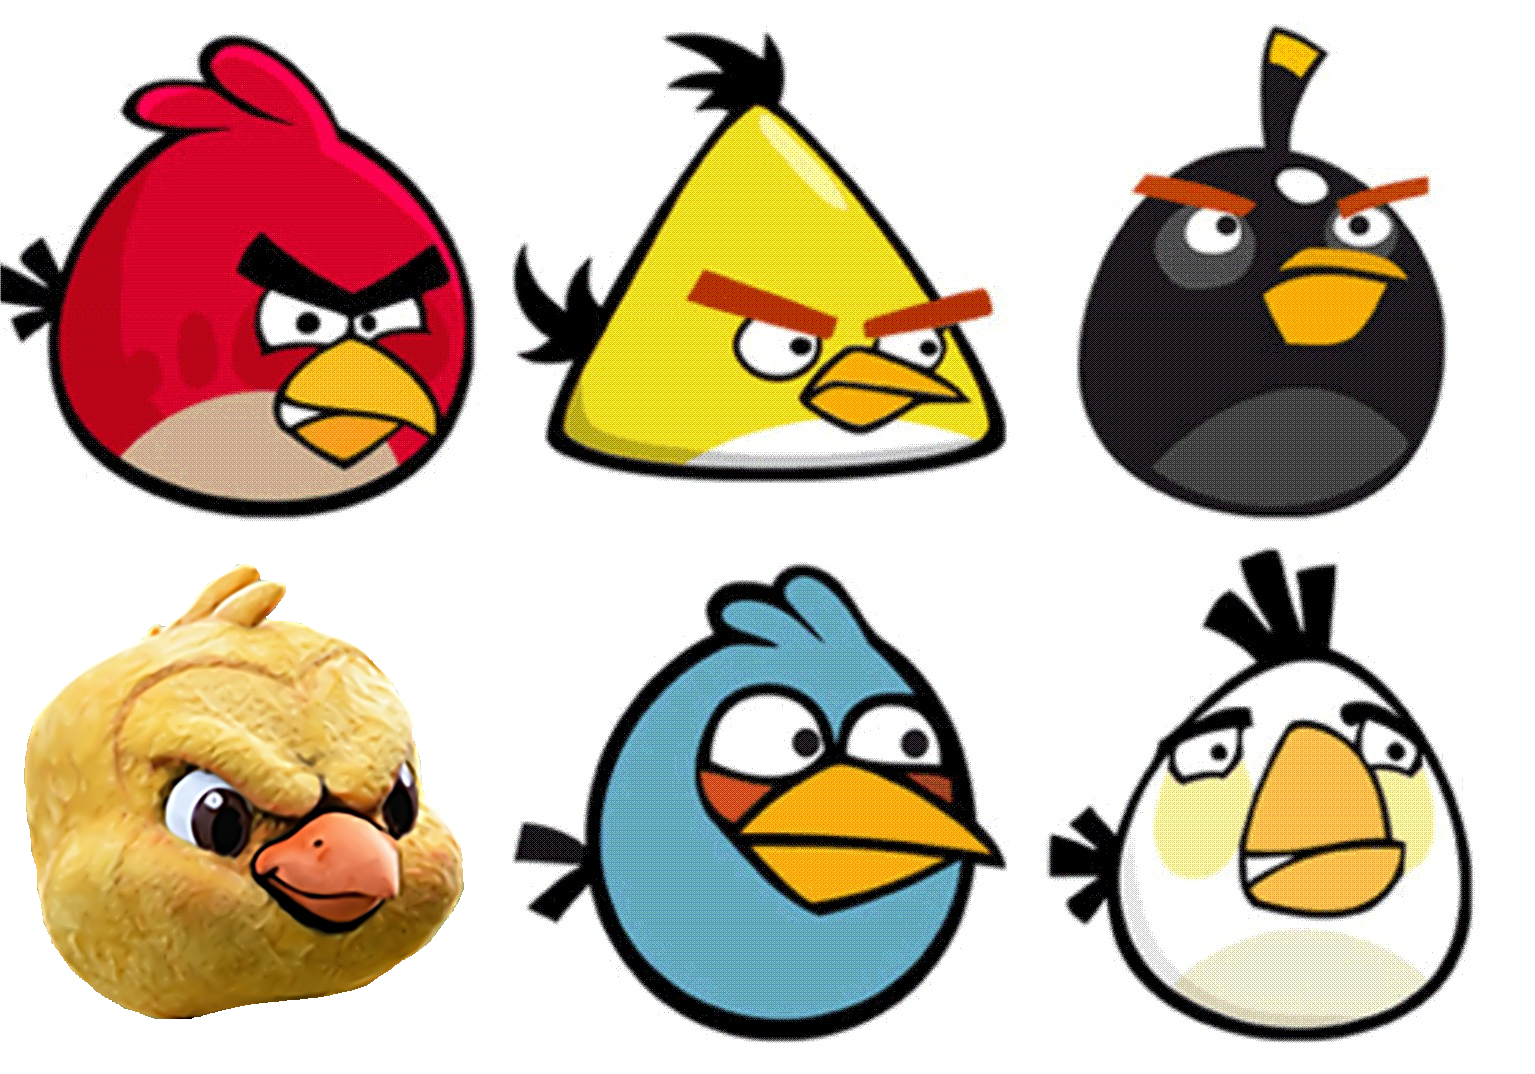
\includegraphics[height=4cm, width=10cm]{Pistola_Birds.png}
\end{center}
\end{figure}
\section{}
\begin{figure}[htbp]
Essa imagem ta com [width=0.7$\backslash$textwidth, angle=30]
\begin{center}
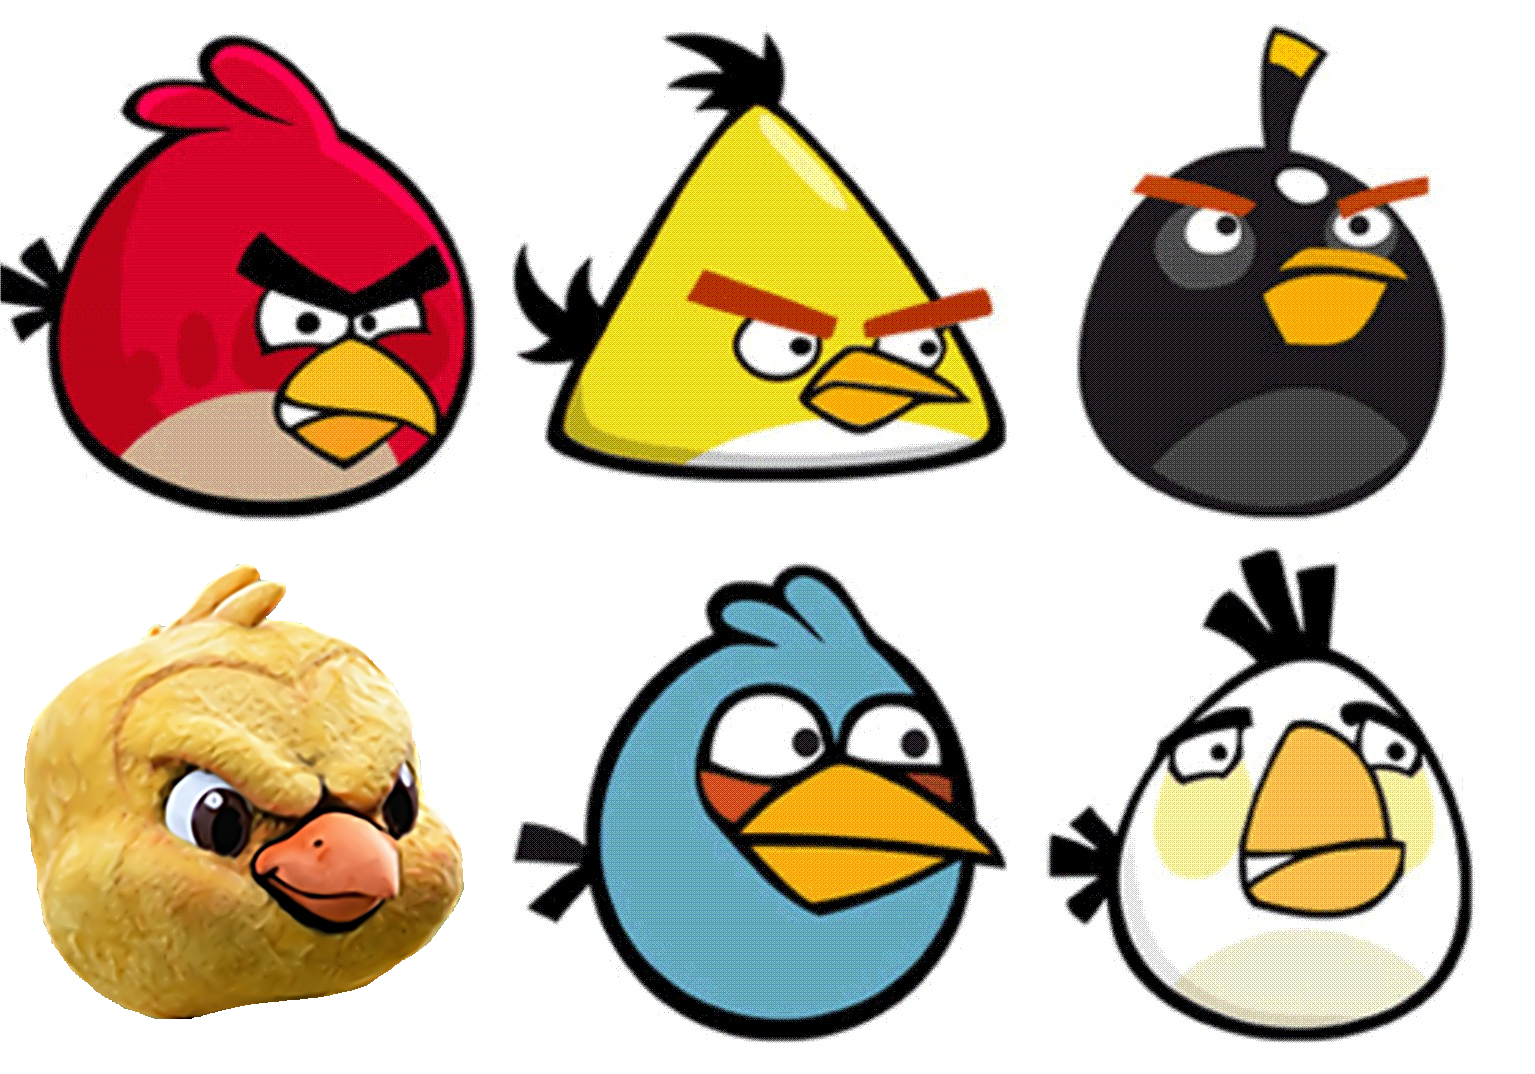
\includegraphics[width=0.7\textwidth, angle=30]{Pistola_Birds.png}
\end{center}
\end{figure}
\begin{figure}[htbp]
\section{}
Essa imagem ta com o ambiente wrapfig
\begin{wrapfigure}{r}{0.5\textwidth}
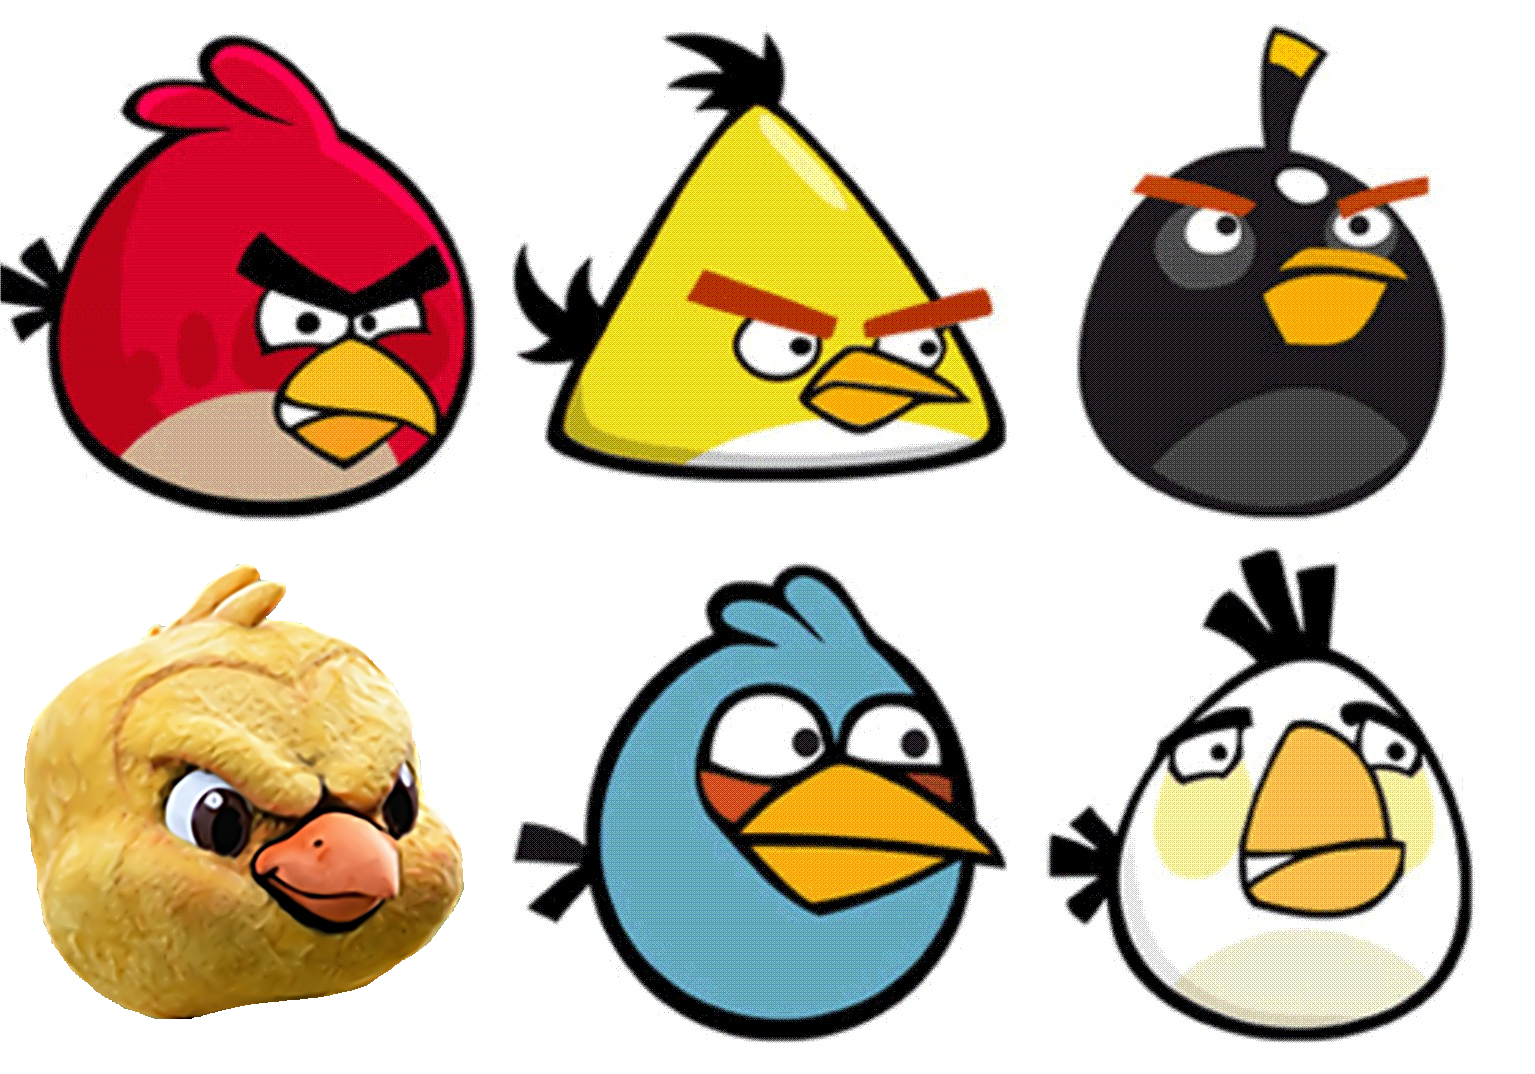
\includegraphics[width=0.5\textwidth]{Pistola_Birds.png}
\end{wrapfigure}

\hspace{.75cm}Nascido na ilha grega de Samos, sua mãe se chamava Pythais e seu pai Mnesarchus era um mercador da cidade de Tiro, além de Pitágoras havia outros dois ou três filhos. Pitágoras passou a infância em Samos embora tenha viajado bastante com seu pai; ele foi treinado pelos melhores professores, alguns deles filósofos. Tocava Lira, aprendeu aritmética, geometria, astronomia e poesia.

\hspace{.75cm}Em cerca de 535 a.C., Pitágoras viajou para o Egito - alguns anos após a ocupação de Samos pelo tirano Policrates - lá, conheceu os templos e aprendeu sobre os sacerdotes locais.

\hspace{.75cm}Em 525 a.C. o rei Persa Cambises I atacou o Egito e Pitágoras foi capturado e enviado para Babilônia (cidade) onde conheceu o sacerdote Mago que o instruiu sobre ensinamentos espirituais.

\hspace{.75cm}Em 522 a.C. ambos Policrates e Sambyses já haviam morrido então Pitágoras retorna a Samos onde funda uma escola de filosofia chamada Semicírculo.

\hspace{.75cm}Por volta de 518 a.C., para evitar conflitos políticos, viaja para o sul da Itália, para a cidade de Crotona onde funda uma escola espiritual,[3] lá, casa-se com Theanos de Creta, filha de Pythenax com quem tem uma filha, Myia.
\end{figure}

\begin{SCfigure}[0.25][h]
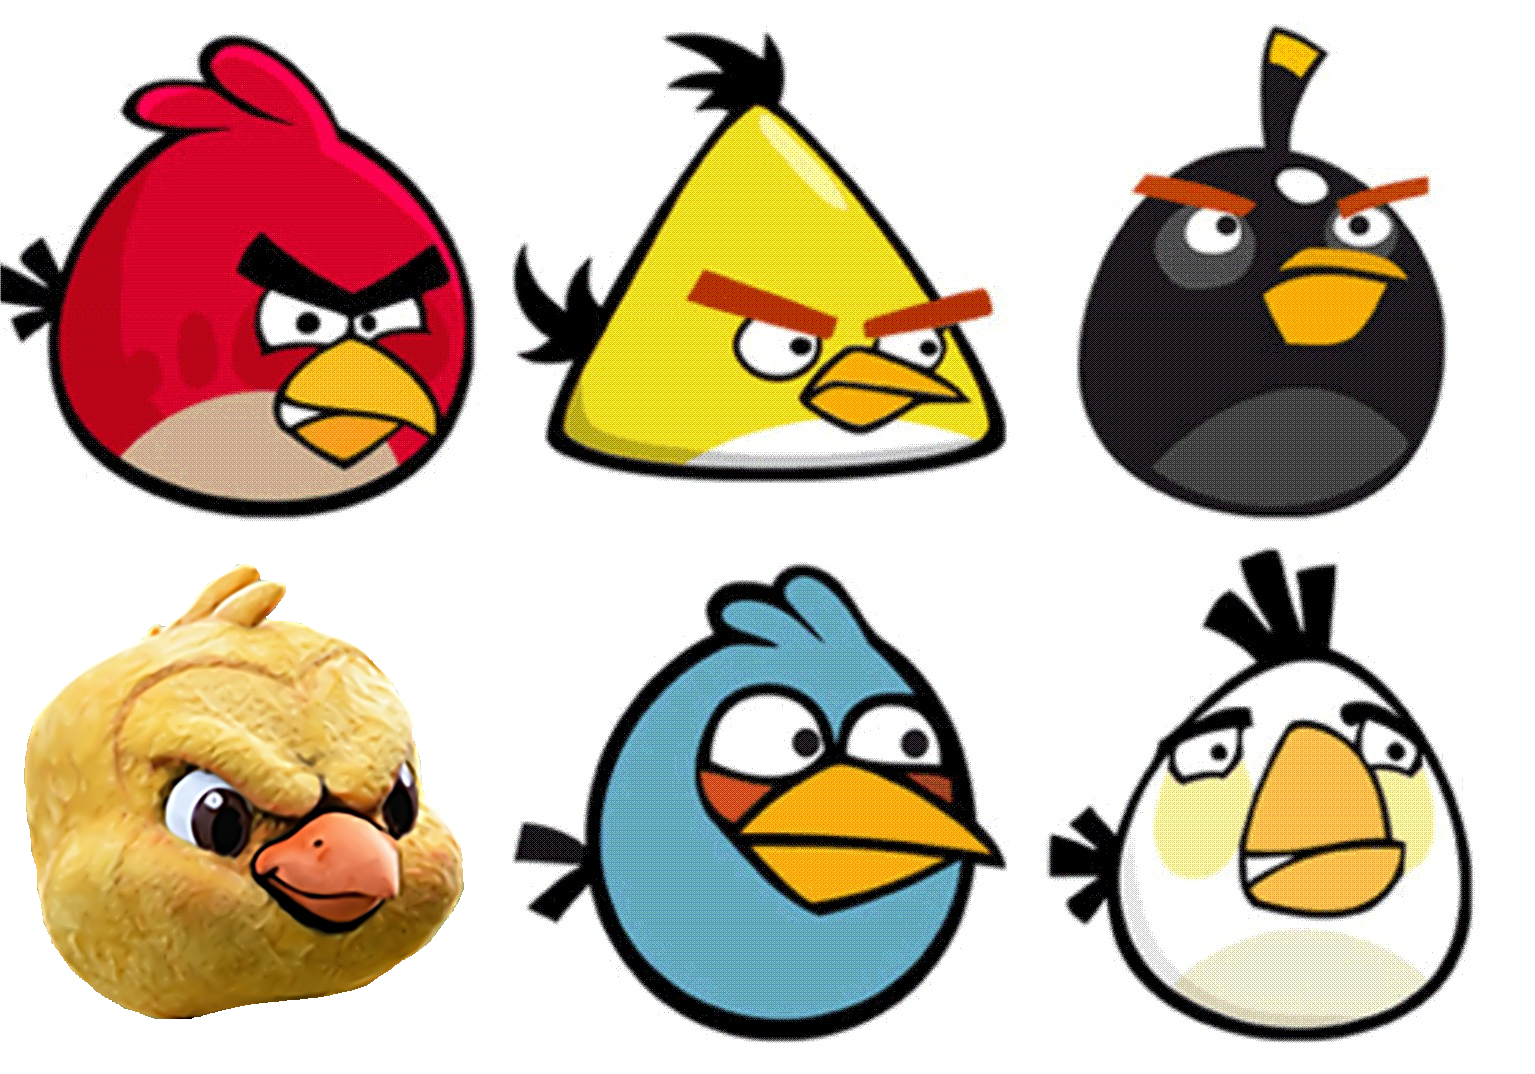
\includegraphics[width=0.5\textwidth]{Pistola_Birds.png}
\caption{Pistola Birds dois}\label{imagemultima}
\end{SCfigure}
%\newpage %porque caralhos isso arrumou tudo?
\chapter{só pra finalizar e testar um bang}
\section{}
As imagens das páginas \pageref{imagemultima} e \pageref{imagemprimeira} estão sendo relembradas com pageref\\
Só pra lembrar pro futuro: usar imagem é uma desgraça\\
\section{}
:)

\end{document}
